\documentclass[border=2pt, 10pt]{standalone}

\usepackage{fontspec}
    \setmainfont{Times New Roman}
\usepackage[dvipsnames]{xcolor}
    \definecolor{GDLcolor}{HTML}{a6a6a6}
    \definecolor{ELcolor}{HTML}{f3f1c5}
    \definecolor{LDLcolor}{HTML}{c5eaf9}
\usepackage{tikz}
    \usetikzlibrary{%
        calc,
        math,
        decorations.pathreplacing, % 画括号的
        decorations.pathmorphing,
        arrows.meta, % 自定义箭头样式
    }
\usepackage{amsmath}

\begin{document}

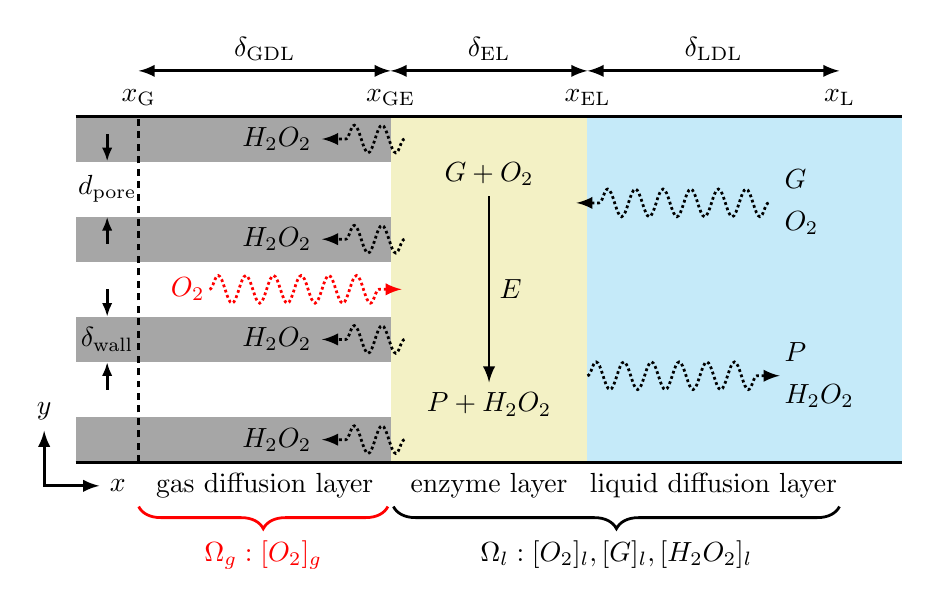
\begin{tikzpicture}[line width=1pt]
    \tikzmath{%
        % 宽
        \deltaGDL=3.2;
        \deltaEL=2.5;
        \deltaLDL=3.2;
        % 高
        \epsilonGDL=0.55;
        \dpore=0.7;
        \deltawall=(1-\epsilonGDL)*\dpore/\epsilonGDL;
        \numwall=4;
        \numpore=\numwall-1;
        \deltafig=\numpore*\dpore+\numwall*\deltawall;
        % 其他元素的长度
        \deltasnake=2.3;
        \offset=0.8;
    };

    \tikzset{%
        snakeline/.pic={%
                \draw [dash pattern=on 1pt off 1pt, color=black, decorate, decoration={snake, amplitude=5pt}] (5pt, 0) -- ++({-\deltasnake/3-0.1}, 0);
                \draw [-latex] (-\deltasnake/3, 0) -- ++(-3pt, 0) node [left] {$ H_2 O_2 $};
            },
    }

    % 定义坐标
    \coordinate (O) at (0, 0); % 原点
    %\fill [red] (O) circle (2pt);
    \coordinate (xG) at ($ (O) + (0, \deltafig) $);
    \coordinate (xGE) at ($ (O) + (\deltaGDL, \deltafig) $);
    \coordinate (xEL) at ($ (O) + (\deltaGDL+\deltaEL, \deltafig) $);
    \coordinate (xL) at ($ (O) + (\deltaGDL+\deltaEL+\deltaLDL, \deltafig) $);
    \coordinate (GDL) at ($ (O) + (\deltaGDL/2, 0) $);
    \coordinate (EL) at ($ (O) + (\deltaGDL+\deltaEL/2, 0) $);
    \coordinate (LDL) at ($ (O) + (\deltaGDL+\deltaEL+\deltaLDL/2, 0) $);

    % axes
    \draw [-latex, line cap=rect] ($ (O) + (-1.2, -0.3) $) -- ++(0.7, 0) node [right] {$ x $};
    \draw [-latex, line cap=rect] ($ (O) + (-1.2, -0.3) $) -- ++(0, 0.7) node [above] {$ y $};

    % GDL
    \foreach \i in {0, ..., \numpore} {%
            \fill [GDLcolor] (-\offset, {\i*(\deltawall+\dpore)}) rectangle ++(\offset+\deltaGDL, \deltawall);
        };
    % EL
    \fill [ELcolor] (\deltaGDL, 0) rectangle ++(\deltaEL, \deltafig);
    % LDL
    \fill [LDLcolor] (\deltaGDL+\deltaEL, 0) rectangle ++(\deltaLDL+\offset, \deltafig);

    % lines
    \draw ($ (O) + (-\offset, 0) $) -- ($ (O) + (\offset+\deltaGDL+\deltaEL+\deltaLDL, 0) $);
    \draw ($ (O) + (-\offset, \deltafig) $) -- ($ (O) + (\offset+\deltaGDL+\deltaEL+\deltaLDL, \deltafig) $);
    \draw [dash pattern=on 2.5pt off 2pt] (O) -- (xG);
    % 侧面node
    \draw [arrows={Latex[length=5pt]}-] ($ (O) + (-\offset/2, \deltawall+\dpore) $) -- ++(0, -10pt);
    \draw [arrows={Latex[length=5pt]}-] ($ (O) + (-\offset/2, \deltawall+\dpore+\deltawall) $) -- ++(0, 10pt);
    \node at ($ (O) + (-\offset/2, 3/2*\deltawall+\dpore) $) {$ \delta_{\mathrm{wall}} $};
    \draw [arrows={Latex[length=5pt]}-] ($ (O) + (-\offset/2, 3*\deltawall+2*\dpore) $) -- ++(0, -10pt);
    \draw [arrows={Latex[length=5pt]}-] ($ (O) + (-\offset/2, 3*\deltawall+3*\dpore) $) -- ++(0, 10pt);
    \node at ($ (O) + (-\offset/2, 3*\deltawall+2*\dpore+0.5*\dpore) $) {$ d_{\mathrm{pore}} $};

    % 顶部node
    \node (xG) [above] at (xG) {$ x_{\mathrm{G}} $};
    \node (xGE) [above] at (xGE) {$ x_{\mathrm{GE}} $};
    \node (xEL) [above] at (xEL) {$ x_{\mathrm{EL}} $};
    \node (xL) [above] at (xL) {$ x_{\mathrm{L}} $};
    \draw [latex-latex] ([yshift=3pt] xG.north) -- ([yshift=3pt] xGE.north)
    node (deltaGDL) [midway, above] {$ \delta_{\mathrm{GDL}} $};
    \draw [latex-latex] ([yshift=3pt] xGE.north) -- ([yshift=3pt] xEL.north)
    node (deltaEL) [midway, above] {$ \delta_{\mathrm{EL}} $};
    \draw [latex-latex] ([yshift=3pt] xEL.north) -- ([yshift=3pt] xL.north)
    node (deltaLDL) [midway, above] {$ \delta_{\mathrm{LDL}} $};

    % 底部node
    \node [below] at (GDL) {gas diffusion layer};
    \node [below] at (EL) {enzyme layer};
    \node [below] at (LDL) {liquid diffusion layer};
    \draw [red, decorate, decoration={brace, mirror, amplitude=8pt}] ($ (xG) + (0, -\deltafig-0.8) $) -- ($ (xGE) + (-1pt, -\deltafig-0.8) $)
    node [midway, below=0.3cm] {$ \Omega_g: [O_2]_g $};
    \draw [decorate, decoration={brace, mirror, amplitude=8pt}] ($ (xGE) + (1pt, -\deltafig-0.8) $) -- ($ (xL) + (0, -\deltafig-0.8) $)
    node [midway, below=0.3cm] {$ \Omega_l: [O_2]_l, [G]_l, [H_2 O_2]_l $};

    % 中间node
    %% O_2 diffusion into EL
    \draw [dash pattern=on 1pt off 1pt, color=red, decorate, decoration={snake, amplitude=5pt}] ($ (O) + (\deltaGDL-\deltasnake, \deltafig/2) $) node [left=-2pt] {$ O_2 $} -- ++(\deltasnake, 0);
    \draw [-latex, color=red] ($ (O) + (\deltaGDL, \deltafig/2) $) -- ++(4pt, 0);
    %% G, O_2 diffusion into EL
    \draw [dash pattern=on 1pt off 1pt, color=black, decorate, decoration={snake, amplitude=5pt}] ($ (O) + (\deltaGDL+\deltaEL+\deltasnake, 3/4*\deltafig) $)
    node [right=2pt] {%
        $
            \begin{aligned}
                 & G   \\
                 & O_2
            \end{aligned}
        $
    } -- ++(-\deltasnake, 0);
    \draw [-latex] ($ (O) + (\deltaGDL+\deltaEL, 3/4*\deltafig) $) -- ++(-4pt, 0);
    % P, H2O_2 out of EL
    \draw [dash pattern=on 1pt off 1pt, color=black, decorate, decoration={snake, amplitude=5pt}] ($ (O) + (\deltaGDL+\deltaEL, 1/4*\deltafig) $) -- ++(\deltasnake, 0)
    node [right=2pt] {%
        $
            \begin{aligned}
                 & P       \\
                 & H_2 O_2
            \end{aligned}
        $
    };
    \draw [-latex] ($ (O) + (\deltaGDL+\deltaEL+\deltasnake, 1/4*\deltafig) $) -- ++(4pt, 0);
    %% G + O_2 -> P + H_2 O_2
    \node (reactants) at ($ (O) + (\deltaGDL+\deltaEL/2, 5/6*\deltafig) $) {$ G + O_2 $};
    \node (products) at ($ (O) + (\deltaGDL+\deltaEL/2, 1/6*\deltafig) $) {$ P + H_2 O_2 $};
    \draw [-latex] (reactants) -- (products) node [midway, right] {$ E $};

    % 加电
    \foreach \i in {0, ..., 3} {%
            \pic at (\deltaGDL, {\deltawall/2+\i*(\deltawall+\dpore)}) {snakeline};
        }
\end{tikzpicture}

\end{document}
